\section{Results}
\label{sec:results}

% Show transferred phase panels when available and a labeled placeholder otherwise.
\newcommand{\resultpanel}[2]{%
  \IfFileExists{#2}{\includegraphics[width=#1]{#2}}{%
    \parbox[c][0.13\textwidth][c]{#1}{\centering\scriptsize [Checkpoint pending]}}}

Unless otherwise stated, quantitative results are summarized over the primary late-training window from iteration 240,000 through 289,900. Values are temporal means with temporal standard deviations in parentheses across 500 observations logged every 100 iterations. These deviations describe fluctuation within one run and are not estimates of between-seed uncertainty. Each configuration was run once; comparisons and rankings are therefore descriptive. The final-window summary over iterations 280,000--289,900 produced the same qualitative ordering and is reported in the supplementary material.

\subsection{Preliminary Effect of Class-Balanced Sampling}

Class-balanced discriminator sampling was selected before the controlled matrix. Relative to the earlier proportional-sampling B00 run, the balanced B00 run increased $r_{\text{sense}}$ from $0.140$ to $0.155$ and $r_{\text{intra}}$ from $0.749$ to $0.839$, while real-fake loss moved from $0.582$ to $0.593$. The Q-objective proxy changed from $0.086$ to $0.089$, and prototype correlation remained $0.703$. Because the proportional and balanced runs were each performed once, terminated at different iterations, and summarized over different late-training windows, this comparison supports balanced sampling as a setup choice but does not provide a seed-replicated estimate of its effect. All subsequent configurations use class-balanced sampling.

\subsection{Fitness Weighting and Gradient Blending}

Table~\ref{tab:late_results} summarizes the controlled $2\times2$ matrix and the three hybrid configurations. The two no-blend cells reveal a tradeoff between the weighting policies. Relative to B00, dynamic weighting in A01 reduced the Q proxy from $0.089$ to $0.062$ and code separation from $0.155$ to $0.088$, while increasing the within-code spread score from $0.839$ to $0.935$ and real-fake loss from $0.593$ to $0.629$. Thus, under the co-adapted metrics used for training, dynamic weighting favored the target within-code spread window and adversarial balance but did not preserve the same degree of code recovery or centroid separation.

In both rows of the factorial matrix, enabling the implemented CA blend reduced the Q proxy. The baseline-weight comparison changed from $0.089$ in B00 to $-0.030$ in A02, and the dynamic-weight comparison changed from $0.062$ in A01 to $-0.066$ in A03. A02 also had the lowest $r_{\text{intra}}$ ($0.619$), whereas A03 retained a high $r_{\text{intra}}$ ($0.883$) despite weak Q recovery and separation. The blend result therefore reproduced directionally under both weighting policies, but Section~\ref{sec:blend_diagnosis} qualifies its interpretation in light of the post hoc implementation audit.

\begin{table*}[t]
\centering
\caption{Late-window BloodMNIST results over iterations 240,000--289,900. Entries are temporal mean (temporal standard deviation) from one run per configuration. Q denotes the weighted Q-objective proxy, PCorr is pixel-space prototype correlation, $\overline{\sigma}$ is PGPE's mean standard deviation, and $\overline{\alpha}$ is the realized blend coefficient. Higher Q, $r_{\mathrm{sense}}$, and $r_{\mathrm{intra}}$ indicate better values under their definitions; lower PCorr indicates less similar code prototypes. Real-fake loss and $\overline{\sigma}$ are diagnostic rather than monotonic quality measures.}
\label{tab:late_results}
\scriptsize
\setlength{\tabcolsep}{3.5pt}
\begin{tabular}{lccccccc}
\toprule
Run & Q proxy & $r_{\text{sense}}$ & $r_{\text{intra}}$ & RFL & PCorr & $\overline{\sigma}$ & $\overline{\alpha}$ \\
\midrule
B00 & $0.089\,(0.002)$ & $0.155\,(0.013)$ & $0.839\,(0.111)$ & $0.593\,(0.014)$ & $0.703\,(0.031)$ & $0.0216\,(0.0005)$ & $0.0000\,(0.0000)$ \\
A01 & $0.062\,(0.008)$ & $0.088\,(0.014)$ & $0.935\,(0.083)$ & $0.629\,(0.018)$ & $0.739\,(0.039)$ & $0.0249\,(0.0003)$ & $0.0000\,(0.0000)$ \\
A02 & $-0.030\,(0.030)$ & $0.102\,(0.024)$ & $0.619\,(0.098)$ & $0.490\,(0.049)$ & $0.697\,(0.056)$ & $0.0340\,(0.0003)$ & $0.0144\,(0.0023)$ \\
A03 & $-0.066\,(0.028)$ & $0.071\,(0.014)$ & $0.883\,(0.074)$ & $0.553\,(0.026)$ & $0.738\,(0.061)$ & $0.0329\,(0.0003)$ & $0.0145\,(0.0018)$ \\
\midrule
A04-hybrid & $0.091\,(0.002)$ & $0.148\,(0.013)$ & $0.894\,(0.106)$ & $0.571\,(0.018)$ & $0.729\,(0.037)$ & $0.0212\,(0.0004)$ & $0.0000\,(0.0000)$ \\
A04-hybrid-v2 & $0.084\,(0.003)$ & $0.136\,(0.012)$ & $0.911\,(0.100)$ & $0.607\,(0.018)$ & $0.746\,(0.037)$ & $0.0222\,(0.0004)$ & $0.0000\,(0.0000)$ \\
hybrid+CA & $0.071\,(0.005)$ & $0.105\,(0.010)$ & $0.741\,(0.112)$ & $0.617\,(0.016)$ & $0.773\,(0.038)$ & $0.0290\,(0.0002)$ & $0.0014\,(0.0012)$ \\
\bottomrule
\end{tabular}
\end{table*}

\subsection{Hybrid Weighting}

The hybrid policy was motivated by the complementary behavior of B00 and A01. It retains the prescribed, health-gated Q-weight trajectory used by the baseline schedule while allowing the adversarial, diversity, separation, and within-code weights to adapt from online metric history. A04-hybrid produced the largest late-window Q proxy observed in the matrix ($0.091$), while retaining $r_{\text{sense}}=0.148$ and increasing $r_{\text{intra}}$ to $0.894$. These values place it near B00 on code recovery and separation and between B00 and A01 on the within-code spread score. This is the best combined configuration observed in the present runs, not a seed-replicated claim of superiority.

A04-hybrid-v2 increased the base adversarial weight from $0.53$ to $0.60$. Its real-fake loss increased from $0.571$ to $0.607$ and $r_{\text{intra}}$ from $0.894$ to $0.911$, while the Q proxy decreased from $0.091$ to $0.084$ and $r_{\text{sense}}$ from $0.148$ to $0.136$. The sensitivity run therefore makes the fitness-budget tradeoff visible: shifting pressure toward adversarial performance did not improve all objectives simultaneously.

The low-dose hybrid+CA run tests whether reducing the nominal blend coefficient from $0.015$ to $0.005$ avoids the degradation observed in A02 and A03. Runtime gating reduced its late-window realized coefficient further to $0.0014$. Nevertheless, relative to A04-hybrid, its Q proxy decreased from $0.091$ to $0.071$, $r_{\text{sense}}$ from $0.148$ to $0.105$, and $r_{\text{intra}}$ from $0.894$ to $0.741$, while $\overline{\sigma}$ remained higher ($0.0290$ versus $0.0212$). The same adverse direction is therefore present at the lower realized dose in this implementation.

\subsection{Exploration Dynamics and Blend Diagnosis}
\label{sec:blend_diagnosis}

Figure~\ref{fig:metric_trajectories} should show that successful no-blend configurations gradually contract their PGPE search distributions. B00, A01, A04-hybrid, and A04-hybrid-v2 begin near $\overline{\sigma}=0.032$ and finish at $0.0208$, $0.0244$, $0.0205$, and $0.0214$, respectively. By comparison, A02 and A03 finish at $0.0339$ and $0.0327$, and hybrid+CA finishes at $0.0286$. The separation appears soon after blend activation in A02 and remains throughout training; A03 is less monotonic but likewise fails to produce sustained contraction.

The CA target diagnostics support a persistent widening tendency independently of blend-altered trajectories. In the four blend-off configurations, $\boldsymbol{\sigma}_{\mathrm{CA}}$ is computed for diagnostics but discarded. The full-run mean sign of $\boldsymbol{\sigma}_{\mathrm{CA}}-\boldsymbol{\sigma}$ is $+0.559$ for B00, $+0.428$ for A01, $+0.611$ for A04-hybrid, and $+0.559$ for A04-hybrid-v2. During the late window, these values increase to $+0.682$, $+0.595$, $+0.721$, and $+0.659$. The widening tendency is therefore a property of the belief-space targets, rather than only a consequence of trajectories already altered by blending.

\begin{figure*}[t]
\centering
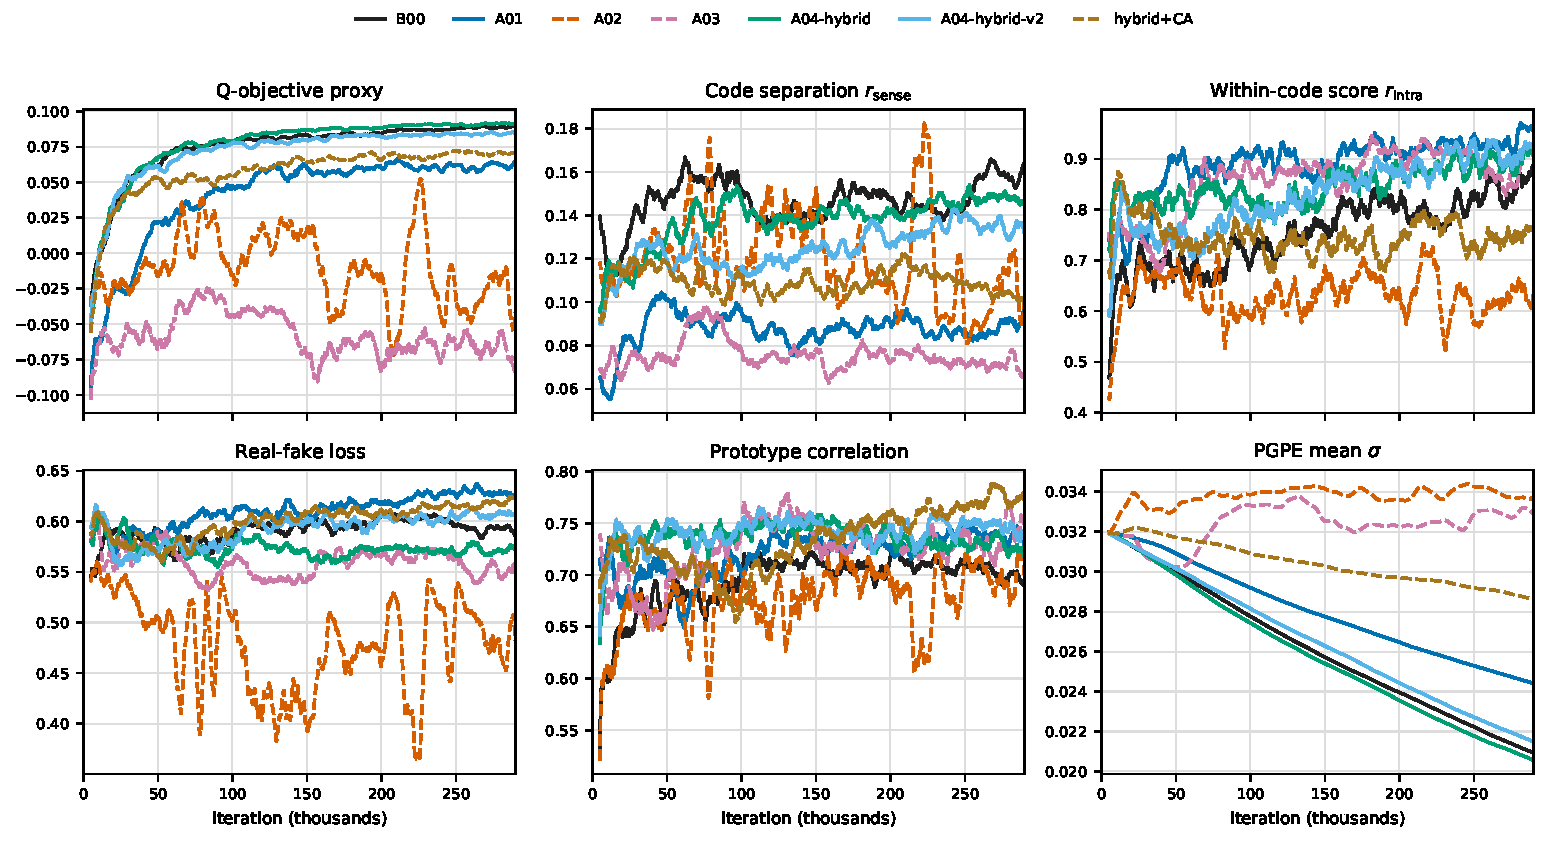
\includegraphics[width=\textwidth]{figures/ablation_metric_trajectories.pdf}
\caption{Training trajectories for the Q-objective proxy, $r_{\text{sense}}$, $r_{\text{intra}}$, real-fake loss, pixel-space prototype correlation, and PGPE mean standard deviation. Curves should use a 5,000-iteration moving average for legibility; all tabulated summaries use unsmoothed observations. Dashed curves denote blend-enabled configurations.}
\label{fig:metric_trajectories}
\end{figure*}

\begin{figure*}[t]
\centering
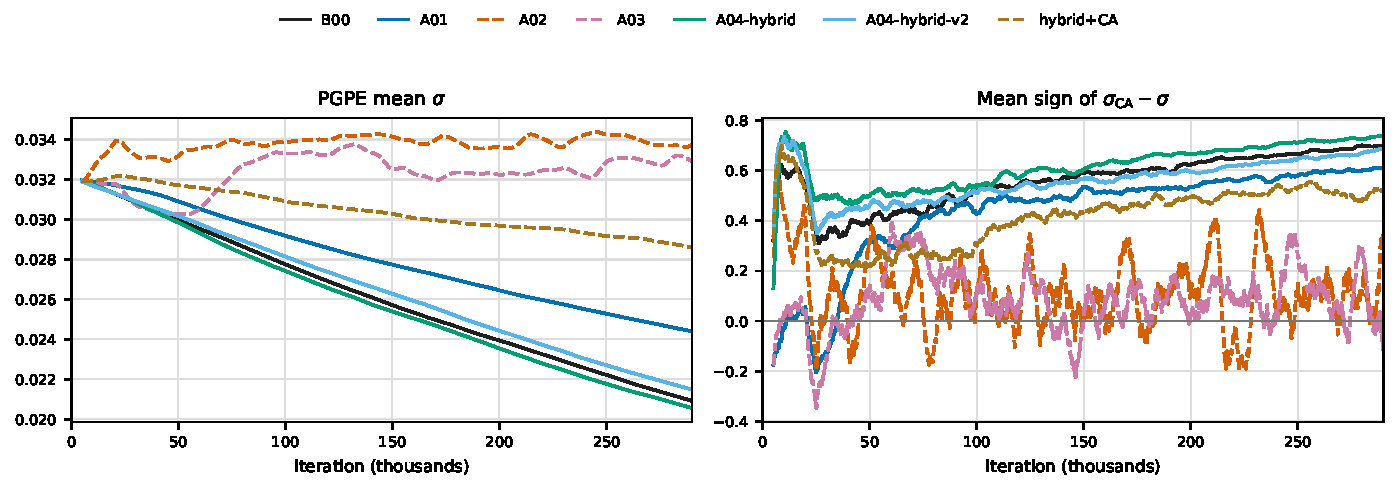
\includegraphics[width=0.92\textwidth]{figures/ca_sigma_diagnostics.pdf}
\caption{CA standard-deviation diagnostics. The first panel shows $\overline{\sigma}$, and the second shows the mean coordinate-wise sign of $\boldsymbol{\sigma}_{\mathrm{CA}}-\boldsymbol{\sigma}$. Positive values indicate that the CA target favors wider exploration. In blend-off runs this direction is diagnostic only; in blend-enabled runs it contributes to the update after norm matching and runtime gating.}
\label{fig:sigma_diagnostics}
\end{figure*}

A post hoc source audit prevents a stronger causal claim. Archive ingestion reconstructed the selected parameter vector using a non-interleaved antithetic indexing assumption, although the sampler emitted positive and negative perturbations in interleaved order. This defect affects CA center guidance but not PGPE's score-function update, the weighting-only runs, or the iteration-level standard-deviation snapshots stored in the archives. The observed widening pressure and stalled contraction therefore support the standard-deviation interaction as the leading explanation for the implemented blend's behavior, but they do not isolate it as the sole cause or establish how a correctly indexed center blend would perform.

\subsection{Fixed Diagnostics and Visual Evaluation}

The fixed image-space diagnostics do not identify a single configuration as semantically disentangled (Table~\ref{tab:morphology_results}). For example, A02 and A03 obtain the highest circularity values, but their saved 100k panels contain smooth, sharply bounded, and often annular structures rather than evidence that their codes correspond to BloodMNIST classes. A03 also has among the lowest cell-area variance values and the lowest nucleus-to-cell ratio range, which is consistent with a restricted template family. These quantities should therefore be read as geometric descriptors rather than monotonic measures of biological quality.

\begin{table*}[t]
\centering
\caption{Fixed pixel-space diagnostics over the late window. Entries are temporal mean (temporal standard deviation). Circularity, area variance, nucleus offset, and nucleus-to-cell ratio range describe generated geometry; no clinically validated target ordering is assumed. PCorr is repeated from Table~\ref{tab:late_results} to connect template similarity to the morphology descriptors.}
\label{tab:morphology_results}
\scriptsize
\setlength{\tabcolsep}{5pt}
\begin{tabular}{lccccc}
\toprule
Run & Circularity & Area variance & Nucleus offset & Nucleus/cell range & PCorr \\
\midrule
B00 & $0.432\,(0.050)$ & $0.003\,(0.001)$ & $0.163\,(0.029)$ & $0.297\,(0.048)$ & $0.703\,(0.031)$ \\
A01 & $0.408\,(0.061)$ & $0.002\,(0.001)$ & $0.152\,(0.032)$ & $0.312\,(0.072)$ & $0.739\,(0.039)$ \\
A02 & $0.501\,(0.100)$ & $0.003\,(0.001)$ & $0.221\,(0.067)$ & $0.231\,(0.045)$ & $0.697\,(0.056)$ \\
A03 & $0.498\,(0.076)$ & $0.001\,(0.000)$ & $0.207\,(0.071)$ & $0.131\,(0.026)$ & $0.738\,(0.061)$ \\
A04-hybrid & $0.441\,(0.050)$ & $0.001\,(0.000)$ & $0.158\,(0.025)$ & $0.186\,(0.041)$ & $0.729\,(0.037)$ \\
A04-hybrid-v2 & $0.452\,(0.061)$ & $0.002\,(0.001)$ & $0.145\,(0.026)$ & $0.204\,(0.041)$ & $0.746\,(0.037)$ \\
hybrid+CA & $0.477\,(0.065)$ & $0.001\,(0.001)$ & $0.147\,(0.029)$ & $0.157\,(0.044)$ & $0.773\,(0.038)$ \\
\bottomrule
\end{tabular}
\end{table*}

The available iteration-100k arrays provide 64 evaluation images per configuration, arranged as eight samples for each of the eight discrete code values. At this checkpoint, B00, A01, A04-hybrid, and A04-hybrid-v2 produce heterogeneous cell-like masses with internal intensity structure. A02, A03, and hybrid+CA show more pronounced smooth contours, rings, and repeated geometric templates. This visual distinction agrees with the quantitative evidence that recoverable code structure need not be biologically meaningful. Because no frozen class or morphology model is used, these observations identify candidate geometric shortcuts and template collapse rather than class-level disentanglement.

Figures~\ref{fig:phase_matrix} and~\ref{fig:phase_hybrids} show the 30k, 100k, and 200k evaluation checkpoints. Each phase panel contains four samples per code, arranged with codes in columns and evaluation repetitions in rows. Each image has its own noise vector; unlike the training metric protocol, noise is not shared across code columns in these saved panels. The same four array positions are retained across phases within each run. Each archived checkpoint contains eight samples per code; selecting the first four repetitions for every run avoids post hoc visual selection.

\begin{figure*}[t]
\centering
\begin{tabular}{c@{\hspace{2pt}}ccc}
& Early (30k) & Middle (100k) & Late (200k) \\
B00 & \resultpanel{0.285\textwidth}{figures/B00_30k_4x8.pdf}
    & \resultpanel{0.285\textwidth}{figures/B00_100k_4x8.pdf}
    & \resultpanel{0.285\textwidth}{figures/B00_200k_4x8.pdf} \\
A01 & \resultpanel{0.285\textwidth}{figures/A01_30k_4x8.pdf}
    & \resultpanel{0.285\textwidth}{figures/A01_100k_4x8.pdf}
    & \resultpanel{0.285\textwidth}{figures/A01_200k_4x8.pdf} \\
A02 & \resultpanel{0.285\textwidth}{figures/A02_30k_4x8.pdf}
    & \resultpanel{0.285\textwidth}{figures/A02_100k_4x8.pdf}
    & \resultpanel{0.285\textwidth}{figures/A02_200k_4x8.pdf} \\
A03 & \resultpanel{0.285\textwidth}{figures/A03_30k_4x8.pdf}
    & \resultpanel{0.285\textwidth}{figures/A03_100k_4x8.pdf}
    & \resultpanel{0.285\textwidth}{figures/A03_200k_4x8.pdf} \\
\end{tabular}
\caption{Qualitative progression for the controlled $2\times2$ matrix. Each panel contains four generated images per code; columns correspond to code values 0--7 and rows to selected evaluation repetitions. Noise vectors differ across cells, so the panels do not implement the shared-$z$ protocol. They support longitudinal comparison and geometric inspection, not supervised class assignment.}
\label{fig:phase_matrix}
\end{figure*}

\begin{figure*}[t]
\centering
\begin{tabular}{c@{\hspace{2pt}}ccc}
& Early (30k) & Middle (100k) & Late (200k) \\
A04-hybrid & \resultpanel{0.26\textwidth}{figures/A04_hybrid_30k_4x8.pdf}
    & \resultpanel{0.26\textwidth}{figures/A04_hybrid_100k_4x8.pdf}
    & \resultpanel{0.26\textwidth}{figures/A04_hybrid_200k_4x8.pdf} \\
A04-hybrid-v2 & \resultpanel{0.26\textwidth}{figures/A04_hybrid_v2_30k_4x8.pdf}
    & \resultpanel{0.26\textwidth}{figures/A04_hybrid_v2_100k_4x8.pdf}
    & \resultpanel{0.26\textwidth}{figures/A04_hybrid_v2_200k_4x8.pdf} \\
hybrid+CA & \resultpanel{0.26\textwidth}{figures/hybrid_CA_30k_4x8.pdf}
    & \resultpanel{0.26\textwidth}{figures/hybrid_CA_100k_4x8.pdf}
    & \resultpanel{0.26\textwidth}{figures/hybrid_CA_200k_4x8.pdf} \\
\end{tabular}
\caption{Qualitative progression for the hybrid configurations, using the same organization as Figure~\ref{fig:phase_matrix}. The comparison isolates the adversarial-weight sensitivity run and the low-dose blend relative to A04-hybrid.}
\label{fig:phase_hybrids}
\end{figure*}

Taken together, the results distinguish an unaffected fitness-level finding from a qualified update-rule finding. The hybrid weighting policy preserved the strongest combined late-window outcome without using archived parameter vectors. The implemented gradient blend was associated with weaker Q recovery and incomplete exploration contraction across all tested weighting contexts, while the audit prevents extending that observation to a correctly indexed center-guidance implementation. Fixed diagnostics and visual panels further show why co-adapted code metrics alone cannot establish hematologically meaningful separation.
